% !TeX spellcheck = en_US

% We need layers to draw the block diagram
\usetikzlibrary{calc,positioning}
\usetikzlibrary{arrows.meta}

% Define a few styles and constants
\tikzstyle{entry}=[draw, minimum height=2em, align=center]
\tikzstyle{mytext}=[align=center]
\tikzstyle{frame} = [entry, text width=29em, fill=white,minimum height=20em, rounded corners]
\tikzstyle{db} = [entry, text width=26em, fill=white,minimum height=6em, rounded corners, left color=green!15!white, right color=green!20!white,shading angle=135, anchor=north]
\tikzstyle{dbentry} = [entry, text width=4em, fill=white,minimum height=3em, rounded corners, left color=blue!15!white, right color=blue!20!white,shading angle=135, anchor=north]
\tikzstyle{overbox} = [entry, text width=6em, shading = axis,rectangle, left color=blue!10!white, right color=blue!30!white,shading angle=135, anchor=north,
minimum height=3em, rounded corners]
\tikzstyle{longbox} = [entry, text width=24em, shading = axis,rectangle, left color=orange!15!white, right color=orange!20!white,shading angle=135, anchor=north,
minimum height=2em, rounded corners]
\tikzstyle{shortbox} = [entry, text width=12em, shading = axis,rectangle, left color=orange!15!white, right color=orange!20!white,shading angle=135, anchor=north,
minimum height=2em, rounded corners]
\tikzstyle{intern} = [entry, text width=8em, shading = axis,rectangle, left color=blue!10!white, right color=blue!30!white,shading angle=135, anchor=north,
minimum height=6em, rounded corners]
\tikzstyle{internr} = [entry, text width=17em, shading = axis,rectangle, left color=blue!10!white, right color=blue!30!white,shading angle=135, anchor=north,
minimum height=6em, rounded corners]
\tikzstyle{corned} = [entry, text width=5em, shading = axis,rectangle, left color=blue!10!white, right color=blue!30!white,shading angle=135, anchor=north,
minimum height=2em, rounded corners]
\def\blockdist{2.3}
\def\edgedist{2.5}

\begin{figure}
	\centering
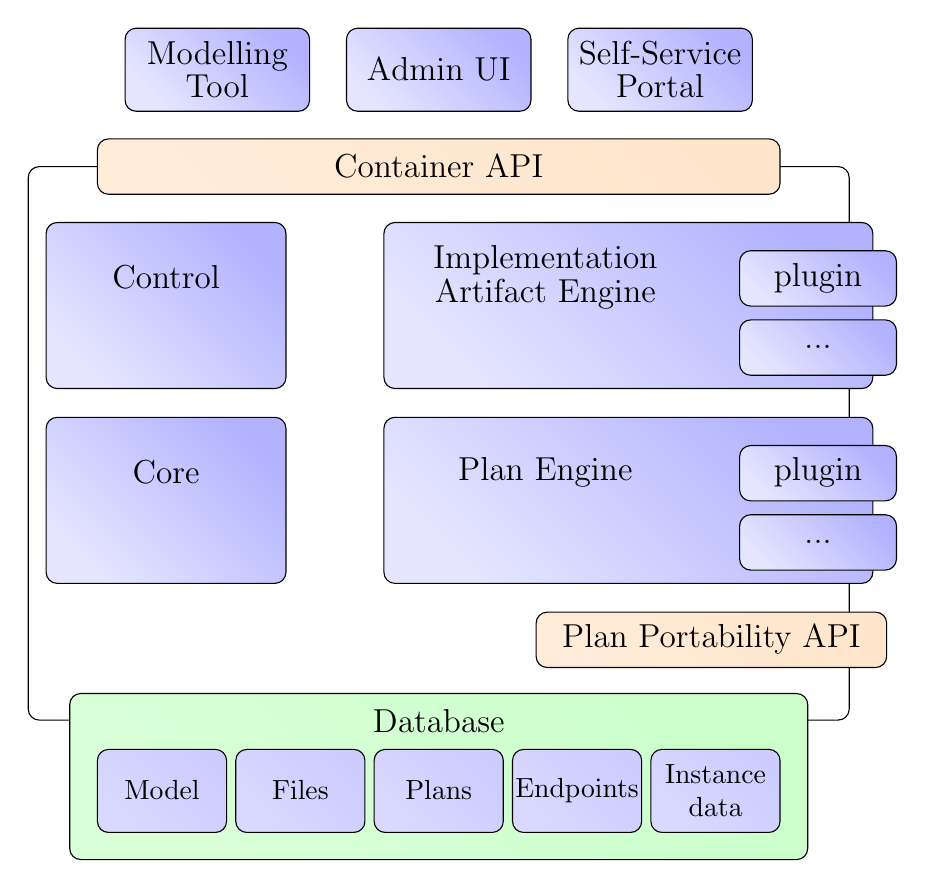
\begin{tikzpicture}
\node (frame) [frame] {};

\node (conapi) [xshift=0em, yshift=+1em] at (frame.north) [longbox] {};
\node at (conapi.north) [yshift=-1em][mytext] {\large Container API};

\node (admininter) [xshift=0em, yshift=+4em] at (conapi.north) [overbox] {};
\node at (admininter.north) [yshift=-1.5em][mytext] {\large Admin UI};

\node (modeltool) [xshift=-8em, yshift=+4em] at (conapi.north) [overbox] {};
\node at (modeltool.north) [yshift=-1.5em][mytext] {\large Modelling\\\large Tool};

\node (selfport) [xshift=+8em, yshift=+4em] at (conapi.north) [overbox] {};
\node at (selfport.north) [yshift=-1.5em][mytext] {\large Self-Service\\\large Portal};

\node (control) [xshift=+5em, yshift=+8em] at (frame.west) [intern] {};
\node at (control.north) [yshift=-2em][mytext] {\large Control};

\node (core) [xshift=+0em, yshift=-1em] at (control.south) [intern] {};
\node at (core.north) [yshift=-2em][mytext] {\large Core};

\node (implart) [xshift=-8em, yshift=8em] at (frame.east) [internr] {};
\node at (implart.north) [xshift=-3em,yshift=-2em][mytext] {\large Implementation\\\large Artifact Engine};

\node (planengine) [xshift=+0em, yshift=-1em] at (implart.south) [internr] {};
\node at (planengine.north) [xshift=-3em,yshift=-2em][mytext] {\large Plan Engine};

\node (pluginimplart) [xshift=-2em, yshift=+2em] at (implart.east) [corned] {};
\node at (pluginimplart.north) [yshift=-1em][mytext] {\large plugin};

\node (dotsimplart) [xshift=-2em, yshift=-0.5em] at (implart.east) [corned] {};
\node at (dotsimplart.north) [yshift=-1em][mytext] {\large ...};

\node (pluginplanengine) [xshift=-2em, yshift=+2em] at (planengine.east) [corned] {};
\node at (pluginplanengine.north) [yshift=-1em][mytext] {\large plugin};

\node (dotsplanengine) [xshift=-2em, yshift=-0.5em] at (planengine.east) [corned] {};
\node at (dotsplanengine.north) [yshift=-1em][mytext] {\large ...};

\node (planport) [xshift=+3em, yshift=-1em] at (planengine.south) [shortbox] {};
\node at (planport.north) [yshift=-1em][mytext] {\large Plan Portability API};

\node (db) [xshift=-0em, yshift=+1em] at (frame.south) [db] {};
\node at (db.north) [yshift=-1em][mytext] {\large Database};

\node (plans) [xshift=-0em, yshift=+1em] at (db) [dbentry] {};
\node at (plans.north) [yshift=-1.5em][mytext] {Plans};

\node (files) [xshift=-5em, yshift=+1em] at (db) [dbentry] {};
\node at (files.north) [yshift=-1.5em][mytext] {Files};

\node (model) [xshift=-10em, yshift=+1em] at (db) [dbentry] {};
\node at (model.north) [yshift=-1.5em][mytext] {Model};

\node (endpoints) [xshift=+5em, yshift=+1em] at (db) [dbentry] {};
\node at (endpoints.north) [yshift=-1.5em][mytext] {Endpoints};

\node (Instancedata) [xshift=+10em, yshift=+1em] at (db) [dbentry] {};
\node at (Instancedata.north) [yshift=-1.5em][mytext] {Instance\\ data};



\end{tikzpicture} 
\caption{OpenTOSCA Architecture} 	\label{fig:openarch}
\end{figure}